\section{Three neutrino effects}
\subsection{Electron neutrino appearance in long baseline experiments}
\label{sec:questdelta}

The measurement of the three large angles $\theta_{12}$,$\theta_{23}$,$\theta_{13}$ opens the possibility of CP violating effects driven by the parameter $\delta_{CP}$. This would be a genuine three neutrino effect: in the following we will explain how these effects can be searched in a long baseline neutrino experiments.

The electron neutrino appearance in a beam of muon neutrino can be written
\begin{eqnarray*}
\papp & = & \sin^2 \theta_{23} \frac{\sin^2 2 \theta_{13}}{(A-1)²} \sin^2 [(A-1) \Delta_{31}] \\
&+& \alpha^2 \cos^2 \theta_{23} \frac{\sin^2 2 \theta_{12}}{A^2} \sin^2 (A\Delta_{31}) \\
&-& \alpha \frac{\sin 2 \theta_{12}\sin 2 \theta_{13}\sin 2 \theta_{23}\cos  \theta_{13}\sin  \delta_{CP}}{A ((1-A)} \sin \Delta_{31} \sin (A\Delta_{31})\sin[ (1-A) \Delta_{31}] \\
&+& \alpha \frac{\sin 2 \theta_{12}\sin 2 \theta_{13}\sin 2 \theta_{23}\cos  \theta_{13}\cos  \delta_{CP}}{A ((1-A)} \cos \Delta_{31} \sin (A\Delta_{31})\sin[ (1-A) \Delta_{31}] \\
\end{eqnarray*}
\begin{equation}
\label{eq:theta13app}
\end{equation}

%\begin{eqnarray*}
%\papp & = & 4C^2_{13}S^2_{13}S^2_{23}\sin^2\phi_{31} \\
%& + & 8 C^2_{13}S_{12}S_{13}S_{23}(C_{12}C_{23} \cos \dcp - S_{12}S_{13}S_{23}) \cos\phi_{32}\sin\phi_{31}\sin\phi_{21} \\
%& - & 8C^2_{13}C_{12}C_{23}S_{12}S_{13}S_{23} \sin \dcp \sin \phi_{32} \sin \phi_{31} \sin \phi_{21} \\
%& + & 4S^2_{12}C^2_{13} (C^2_{12}C^2_{23} + S^2_{12}S^2_{23}S^2_{13} - 2C_{12}C_{23}S_{12}S_{23}S_{13} \cos \dcp ) sin^2\phi_{21}\\
%& - & 8C^2_{13} S^2_{13} S^2_{23} \frac{aL}{4E_{\nu}} (1 - 2S^2_{13} ) \cos\phi_{32} \sin \phi_{31} \\
%& + & 8C^2_{13}S^2_{13}S^2_{23}\frac{a}{\dmsqtwo}(1-2S^2_{13})\sin^2\phi_{31} \\
%\end{eqnarray*}
%\begin{equation}
%\label{eq:theta13app}
%\end{equation}
where $ \alpha = \Delta m^2_{21} / \Delta m^2_{31}$, $\Delta_{ij}= \Delta m^2_{ij} L / 4 E$, $A= 2\sqrt 2 G_F n_e E/ \Delta m^2_{31}$.
%where $C_{ij} = \cos \theta_{ij}$, $S_{ij} = \sin \theta_{ij}$ and $\phi_{ji}~= \Delta m^2_{ji} L / 4 E_{\nu}$. The terms that include $a$ are a consequence of the matter effects with $a=2\sqrt 2 G_F n_e E_{\nu}~=~7.56\times10^{-5} [eV^2](\rho/(g/cm^3)(E_{\nu}/GeV)$. 
The equivalent term for \pappb can be obtained by reversing the signs of the terms proportional to sin\dcp and to $A$. 

The first term in this equation is the leading order term and corresponds to the 3-1 sector oscillation driven by the atmospheric $\Delta m^2_{31}$. It should be noticed that it contains also a factor $\sin^2 \theta_{23}$ that is sensitive to the octant, while the leading order term in $\nu_\mu$ survival probability for atmospheric neutrino and long baseline experiments contains a factor $\sin^2 2 \theta_{23}$. In principle a precise determination of the appearance probability allows therefore to determine the octant of $\theta_{23}$.

The second term corresponds to the 2-1 sector oscillation and is suppressed because of the smallness of $ \alpha \simeq 0.03$. In other terms, for 
$\Delta m^2_{31} L / 4 E \simeq \pi/2$ which is the working point usually adopted for long baseline experiments, the phase $\Delta m^2_{21} L / 4 E$ is lagging behind.

The third term contains the CP violating part and is proportional to the Jarlskog invariant $J=C^2_{13}C_{12}C_{23}S_{12}S_{13}S_{23} \sin \dcp $. It modifies the leading order term by as much as $\pm$ 30 \% for $\dcp = \mp 30 \%$ respectively.

The fourth term is CP conserving but contains a different dependence  on $\delta_{CP}$  as  $\cos \delta_{CP}$: it might therefore be useful for resolving degeneracies. As this term is proportional to $\cos \Delta_{31}$, it is zero for $\Delta_{31}=\pi/2$. It must therefore be studied for L/E away from the first oscillation maximum. 

Matter effects enter through the $A$ term. It can be seen that $A$ is proportional to the $E/E_{res}$, where $E_{res}$ is the energy for which the resonance condition is attained in the medium of constant density. Since the resonance condition can be satisfied either for neutrinos or for antineutrinos, depending on the sign of $\Delta m^2_{31}$ and therefore on the mass ordering, matter effects either enhance $ P (\nu_\mu \rightarrow \nu_e)$ or  $ P (\bar{\nu}_\mu \rightarrow \bar{\nu}_e)$. 
An estimate of $A$ for the various long baseline experiments is shown in Table~\ref{tab:mateff}.
It can be seen that the matter effects are very small for T2K, sizeable for \nova and even more important for DUNE, as they enter non-linearly through the factor $1/(1-A)^2$ in the first term of Eq.~\ref{eq:theta13app}.

\begin{table}
\caption{Matter effect parameter A for various baselines and energies for a constant matter density of 2.6 g/cm$^{-3}$.}
\centering
\begin{tabular}{|c|c|c|c|}
  \hline
  Experiment & L & E & A  \\ 
  \hline
  T2K & 295 & 0.6 & 0.046 \\
  \nova & 800 & 1.6 & 0.12\\
  DUNE & 1300  & 2.6  & 0.20 \\
  T2KK & & & \\
  \hline
\end{tabular}

\label{tab:mateff}
\end{table}


On the other hand CP violating effects also enhance either the neutrino or the antineutrino appearance probability. In summary then, a precise measurement of 
$ P (\nu_\mu \rightarrow \nu_e)$ and  $ P (\bar{\nu}_\mu \rightarrow \bar{\nu}_e)$
would allow the determination of the remaining unknowns in the PMNS matrix, that is: the octant of $\theta_{23}$, $\delta_{CP}$ and the mass ordering, together with an independent determination of $\theta_{13}$, which explains why long baseline neutrino experiments capable of carrying out this experimental program have received a lot of attentions in the last years. 


\begin{figure} [htbp!]
\begin{center}
%add plot!!!
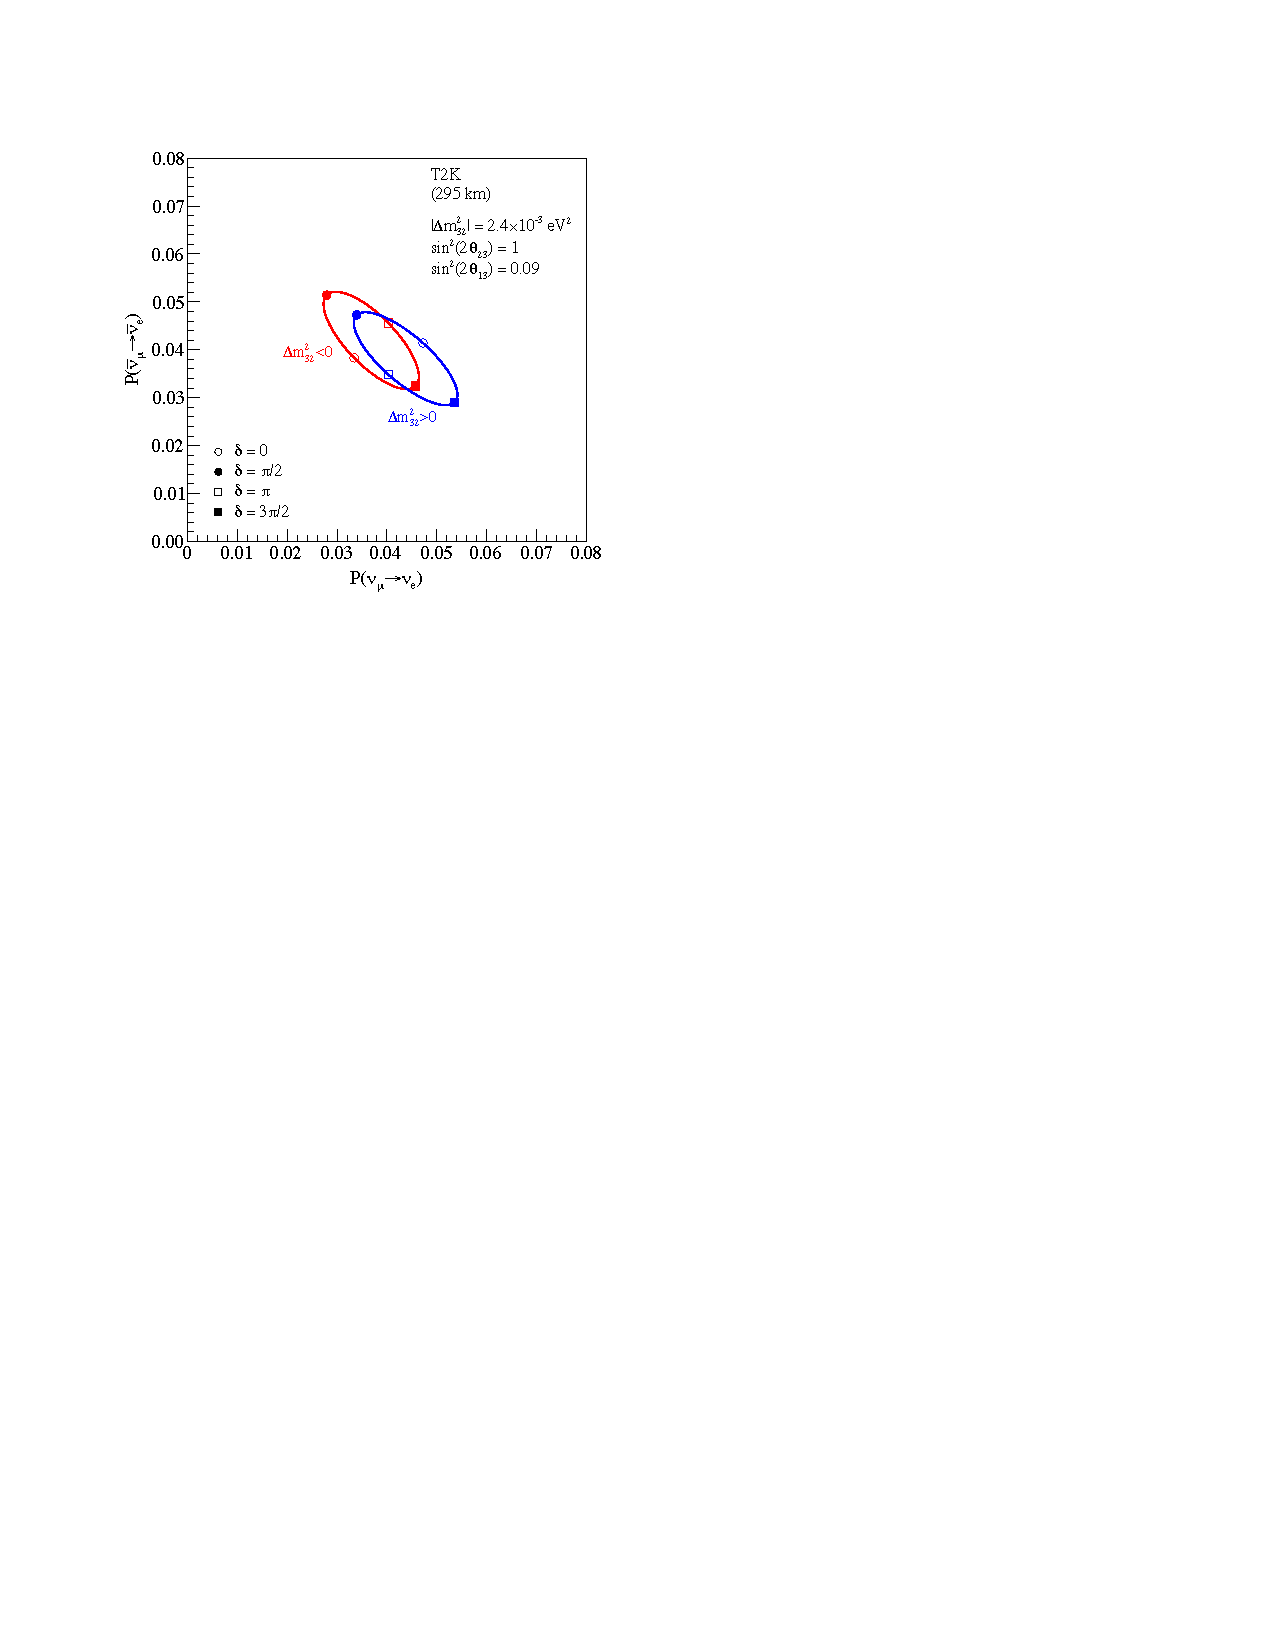
\includegraphics[width=6cm]{figures/t2k_ellipse.pdf}
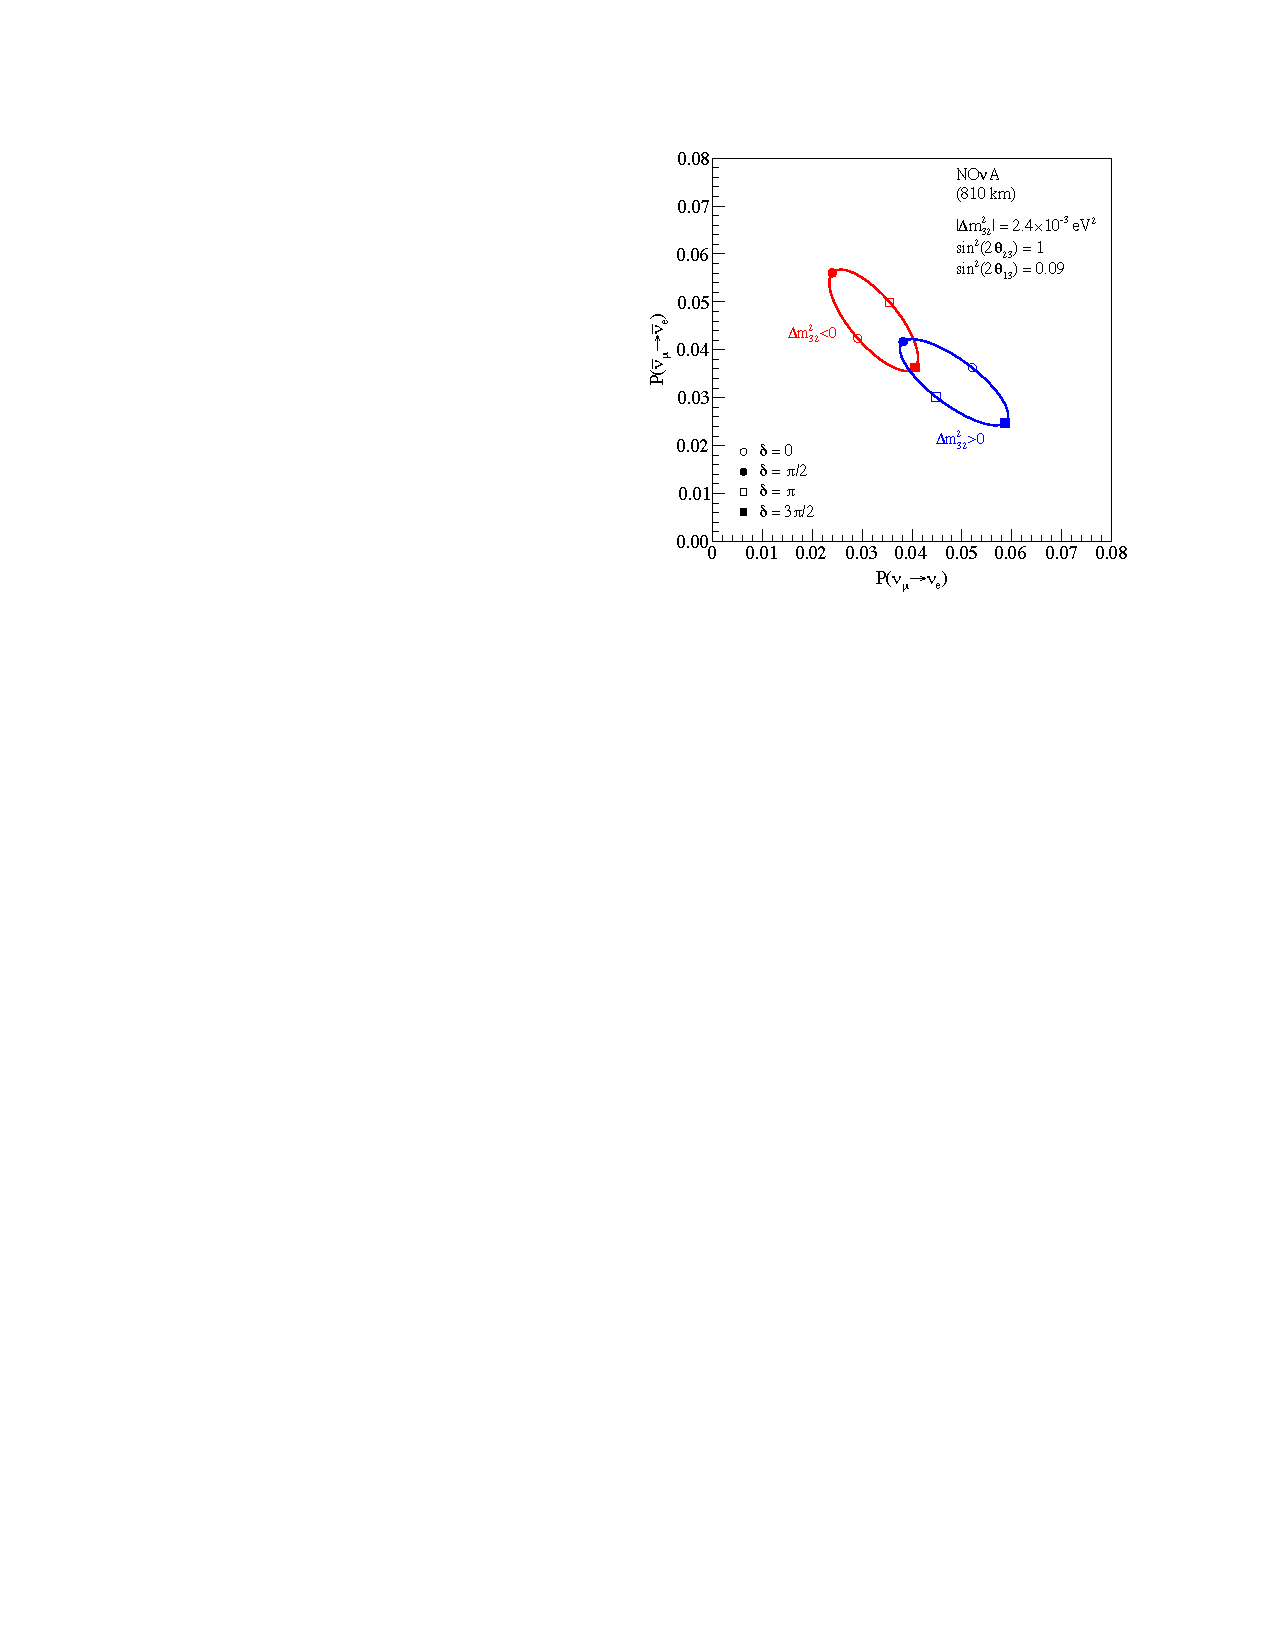
\includegraphics[width=6cm]{figures/nova_ellipse.pdf}
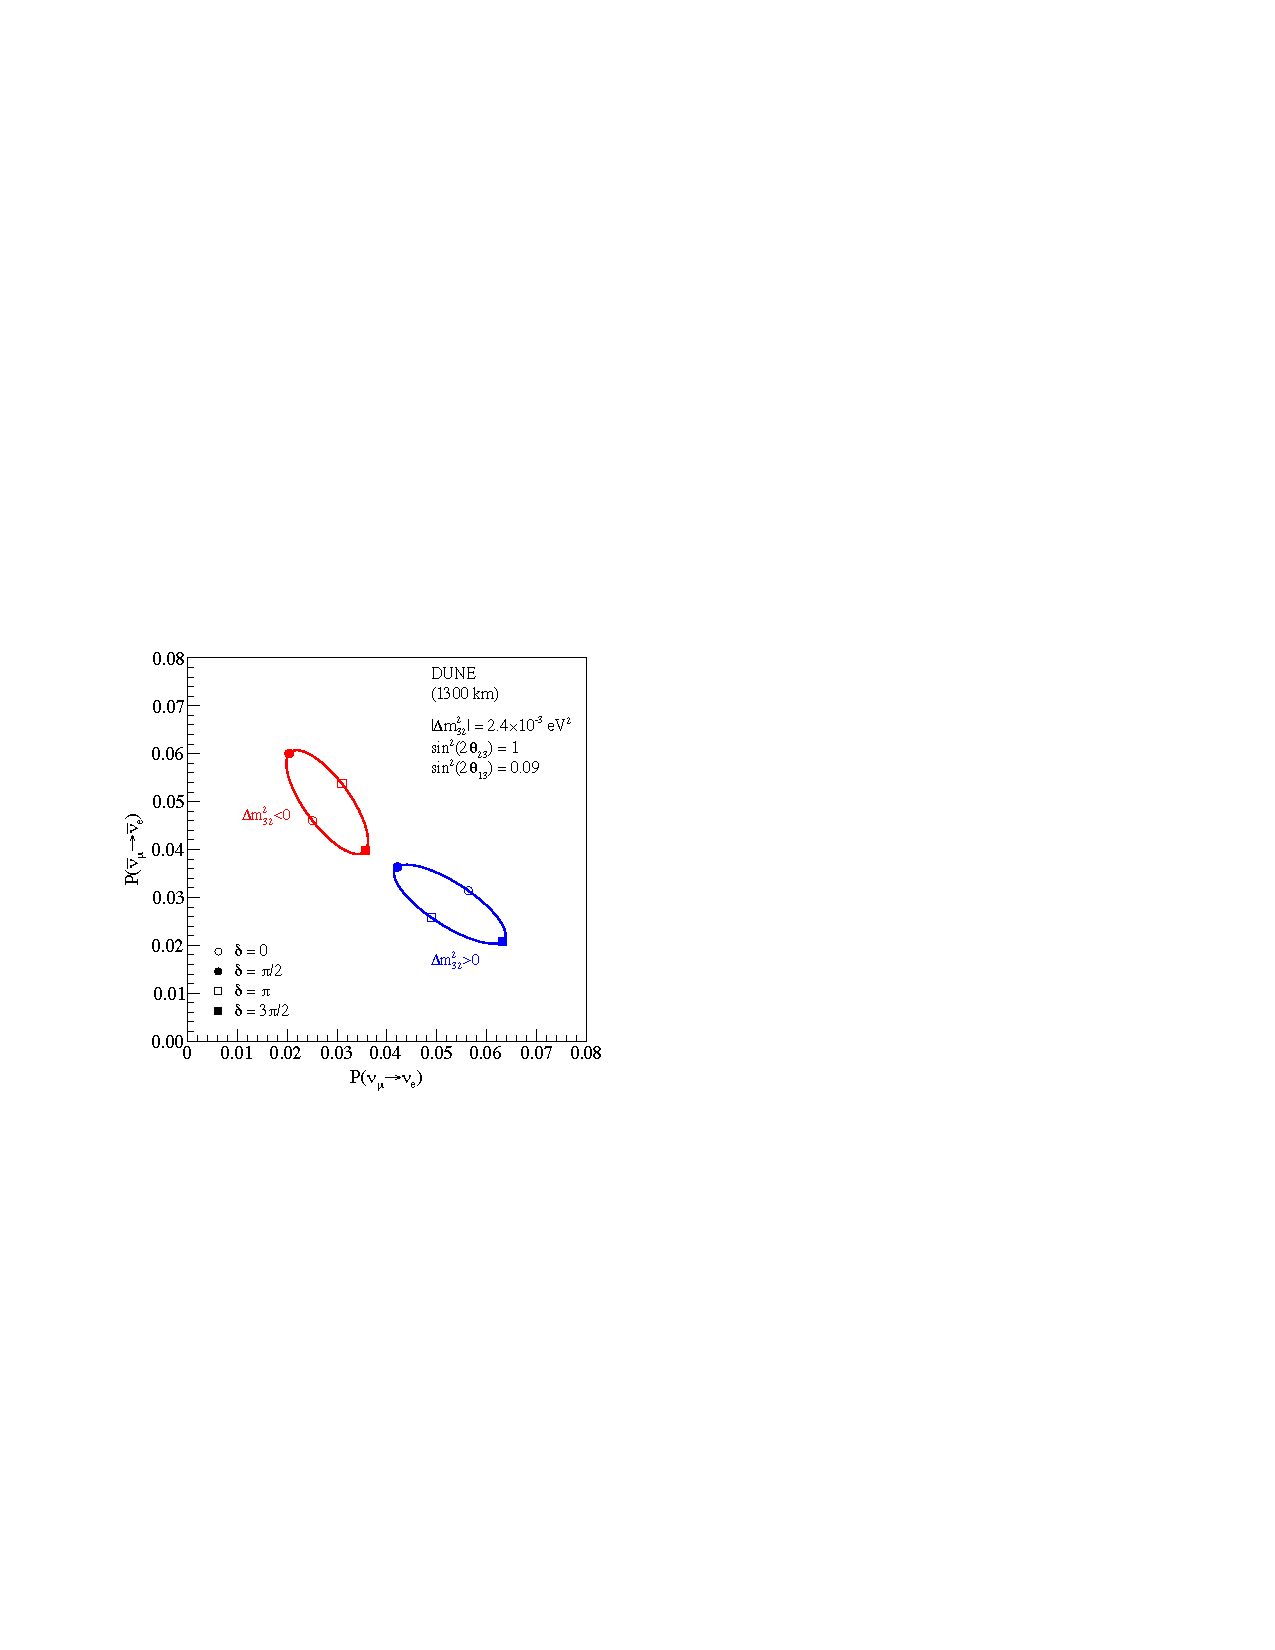
\includegraphics[width=6cm]{figures/dune_ellipse.pdf}
\caption{\label{fig:novaellipse} $ P (\nu_\mu \rightarrow \nu_e)$ versus  $ P (\bar{\nu}_\mu \rightarrow \bar{\nu}_e)$ for T2K (left), \nova (center), and DUNE (right) baselines for a representative L/E value of 0.4 km/MeV~\cite{Patterson:2015xja}.}
\end{center}
\label{fig:biprob}
\end{figure}

The interplay of the various terms of Eq.~\ref{eq:theta13app} can best be understood by considering the plane $ P (\nu_\mu \rightarrow \nu_e)$ versus  $ P (\bar{\nu}_\mu \rightarrow \bar{\nu}_e)$ shown in Fig.~\ref{fig:biprob} for a fixed L and E. The leading order term always lies on the diagonal. The CP-violating third term and the CP-conserving fourth term modulate the bi-probability in the shape of an ellipse as a function of \dcp.
Matter effects displaces this ellipse either enhancing $ P (\nu_\mu \rightarrow \nu_e)$ or 
$ P (\bar{\nu}_\mu \rightarrow \bar{\nu}_e)$.


It has been pointed out that this experimental program is actually more difficult because of multiple degeneracies~\cite{burguet,parkedeg}. Even a measurement of $ P (\nu_\mu \rightarrow \nu_e)$ and  $ P (\bar{\nu}_\mu \rightarrow \bar{\nu}_e)$ with infinite precision at a single energy and baseline would lead to multiple ambiguities in the determination of the underlying parameters. In practice, lifting these degeneracies will be obtained by comparing measurement at different baselines, like T2K and \nova for the running experiments, or DUNE and Hyper-Kamionande in the next decade. Moreover, both DUNE and Hyper-Kamiokande are considering multiple L/E within the same experiment. DUNE will achieve this with a wide-band beam, capable of some sensitivity at the second oscillation maximum. Hyper-Kamiokande is considering a second detector on the same beam line but at a very different L. A precise determination of $\theta_{23}$ becomes increasingly difficult if the true value lies very close to $\pi/4$~\cite{parkedeg}. 

%The term proportional to cos\dcp is invariant for $\nu$ and \nub whilst the term proportional to sin\dcp contains the CP violating part and is proportional to the Jarlskog invariant $J=8C^2_{13}C_{12}C_{23}S_{12}S_{13}S_{23} \sin \dcp $ (verifier). 

%The different terms contributing to \papp are plotted in Fig~\ref{fig:t2kappprob}.
%The relative size of the effect on the appearance probability due to \dcp and to the mass ordering depends on the baseline. 
%The matter effects enhance the appearance probability for neutrinos and reduce it for antineutrinos, depending on mass ordering (Fig.~\ref{fig:t2kappnub}). Therefore there is a degeneracy between mass ordering and CP violation effect at shorter baselines. This degeneracy can be lifted either by performing measurements at very long baselines or by measuring the mass ordering in a different experiment, as explained later~\ref{sec:future}.

\begin{figure} [htbp!]
\begin{center}
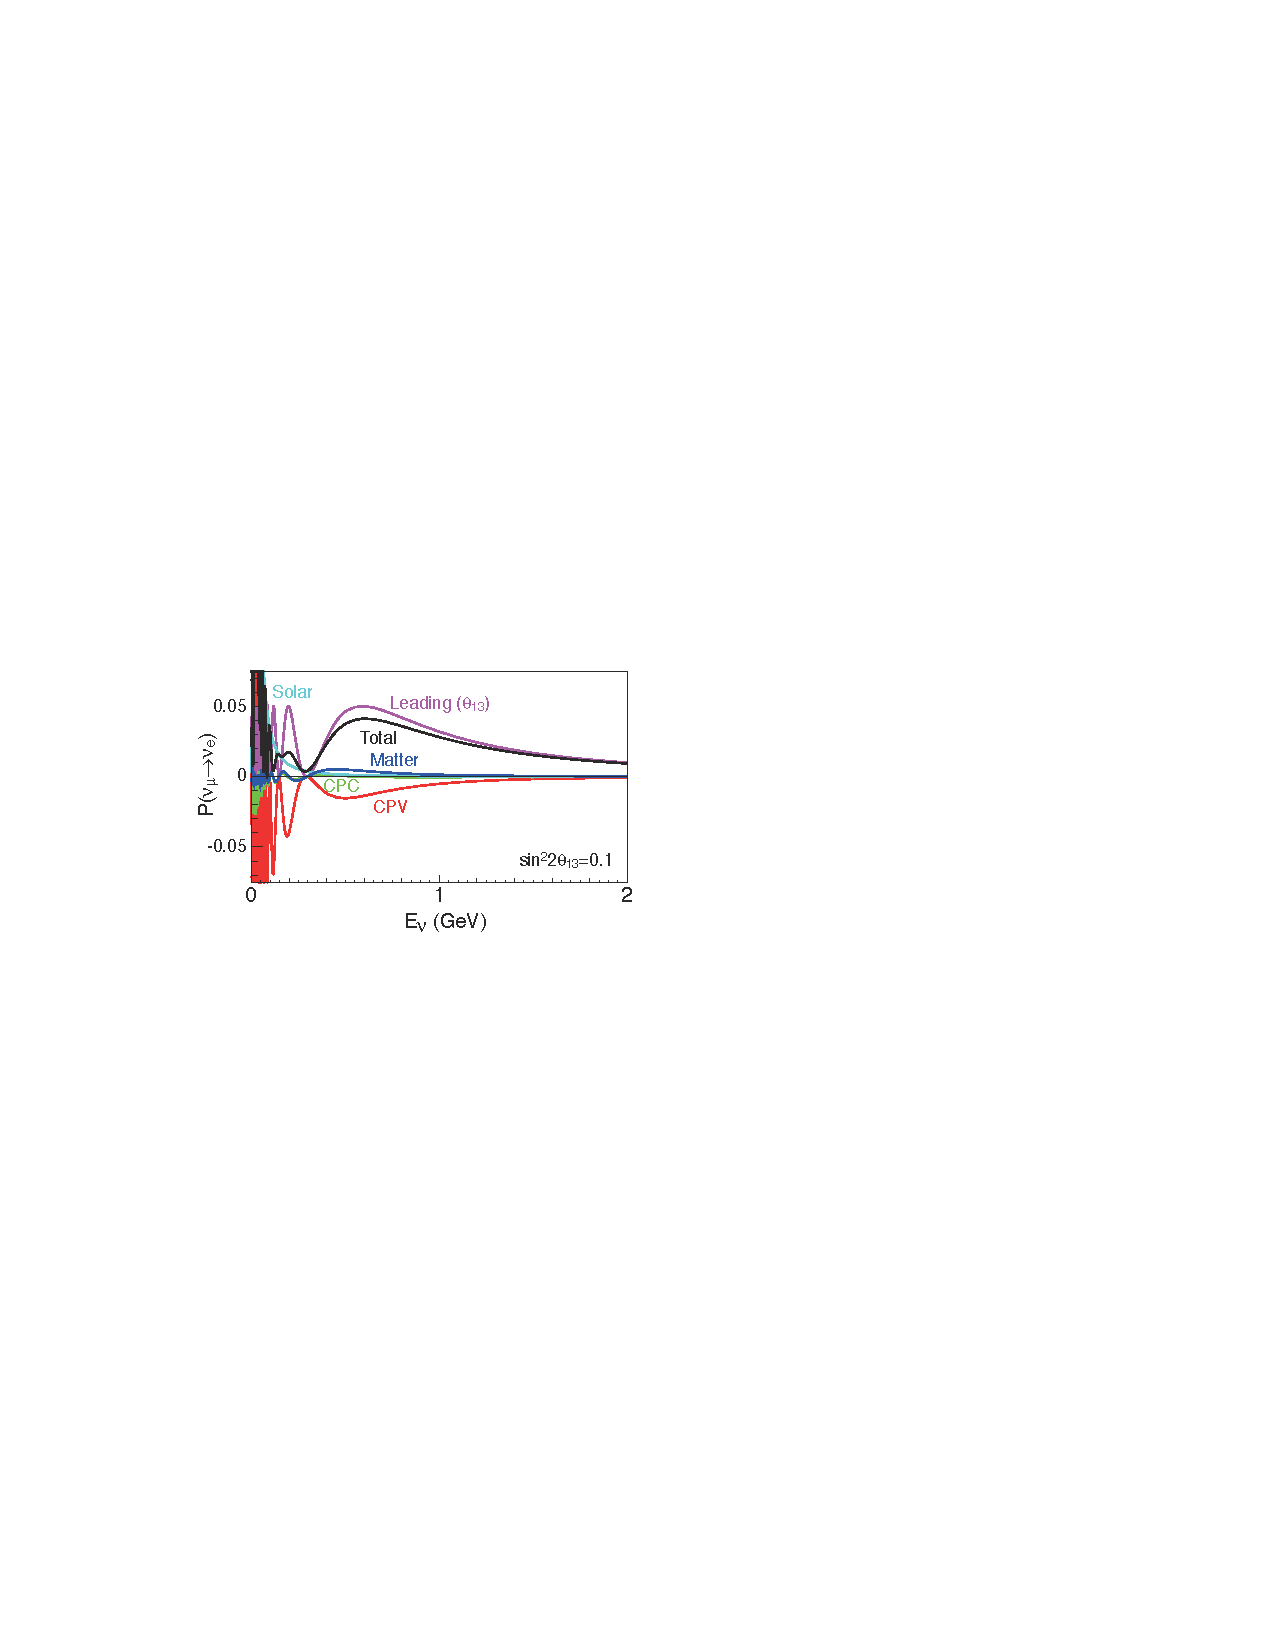
\includegraphics[width=8cm]{figures/papp_prob_2.pdf}
\caption{\label{fig:t2kappprob} Oscillation probabilities as a function of neutrino energy with L=295 km, \stot = 0.1, \dcp=$\pi/2$ and normal hierarchy. The contribution of the different terms of the oscillation probability is shown separately.}
\end{center}
\end{figure}


%\begin{figure} [htbp!]
%\begin{center}
%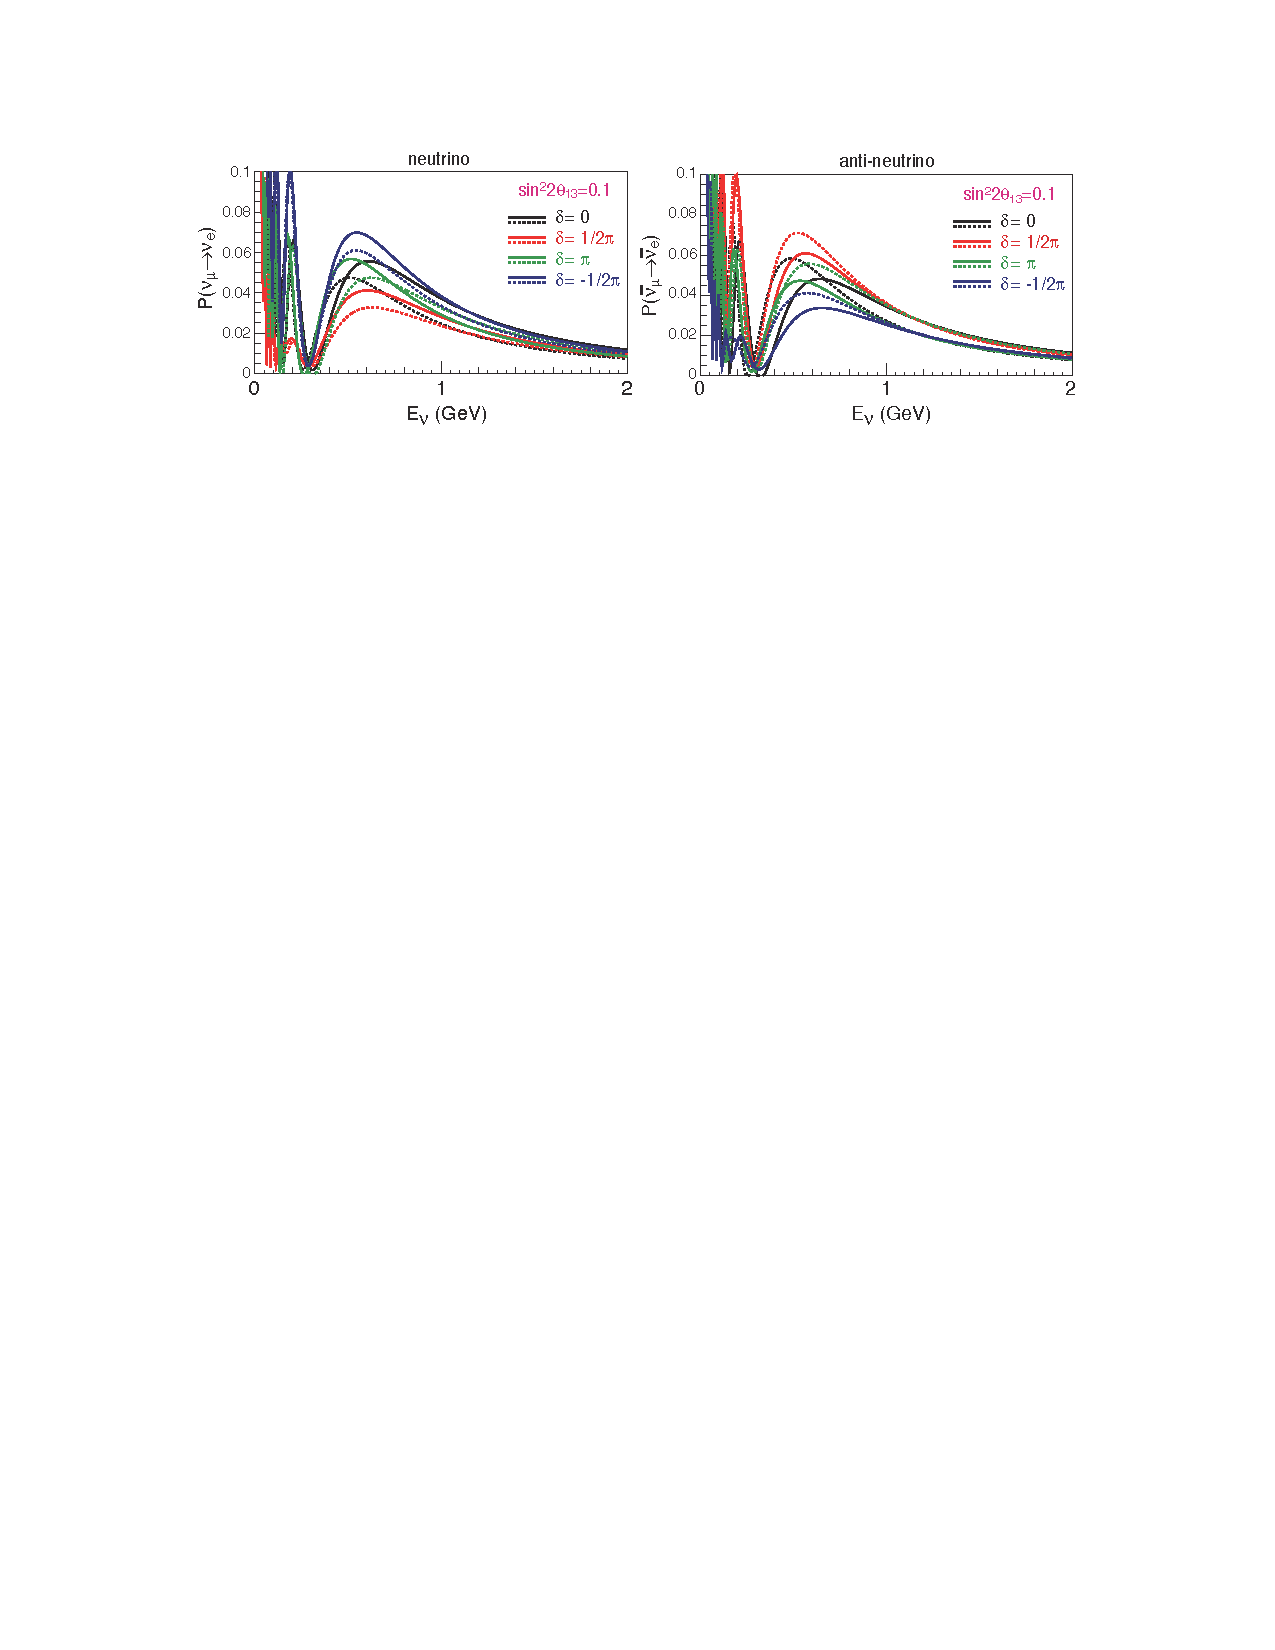
\includegraphics[width=14cm]{figures/papp_prob.pdf}
%\caption{\label{fig:t2kappnub} Oscillation probabilities as a function of neutrino energy for \papp (left) and \pappb (right) with L=295 km and \stot = 0.1. The different line colors correspond to different values of \dcp while the solid (dashed) lines represent the normal (inverted) hierarchy.   }
%\end{center}
%\end{figure}

%\begin{figure} [h!]
%\begin{center}
%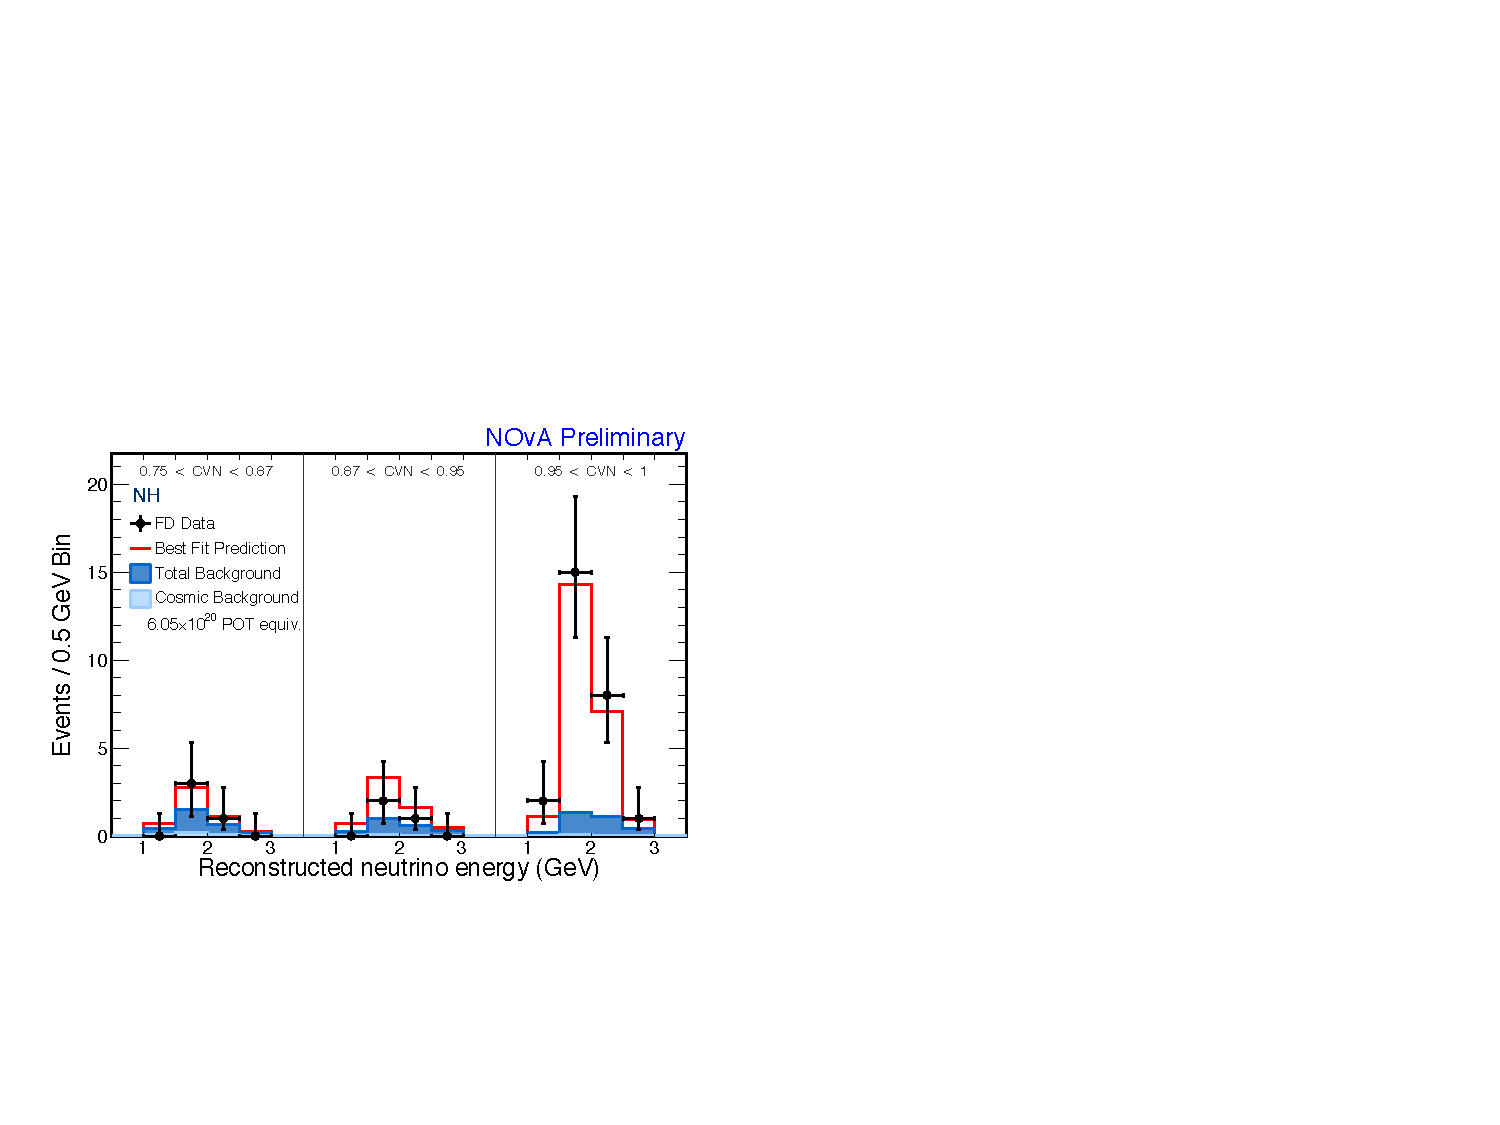
\includegraphics[width=8cm]{figures/nueapp_NOVA.pdf}
%\caption{\label{fig:novaapp} Reconstructed neutrino energy for \nue candidates in \nova in three bins of the Convolutional Visual Network (CVN) discrimination variable.}
%\end{center}
%\end{figure}
%
%In principle, a precise measurement of $Prob(\nu_\mu \rightarrow \nu_e$ and 
%$Prob(\bar{\nu}_\mu \rightarrow \bar{\nu}_e$ allows to determine all the remaining unknown parameters related to the neutrino oscillation, namely: the angle
%$\theta_{13}$ (appears in the leading term of Eq.\ref{eq:theta13app}), the octant of $\theta_{23}$ (the leading term of Eq.\ref{eq:theta13app} being proportional to $\sin (\theta^2_{23}$), the CP violation phase $\delta$ and the mass ordering from matter effects. 

%The combination of experiments with different baselines is particularly useful as it allows to remove degeneracies among the parameters.
%Indeed, in the case of T2K the baseline is relatively short (295 km) and the matter effects contribute to $\sim\pm10\%$ of the oscillation probability while the effect due to \dcp can be as large as $\pm30\%$ for the extreme values of \dcp as shown in Fig.~\ref{fig:t2kappprob}. In the case of NOVA the baseline is 810 km and the effect of the mass ordering and of \dcp on \papp is roughly equal and it corresponds to $\sim20\%$ for each source.
%
%At the moment, the precision of the long baseline results is insufficient to completely carry out this program and the precise measurement of \nueb disappearance with reactors is still needed to extract information on the sub-leading terms entering the appearance probability, particularly the CP violation term \dcp and the mass ordering. 

%It is important to notice that for \nueb appearance the signs are reverted. In neutrino mode the appearance probability is maximized for normal hierarchy and $\dcp=-\pi/2$ while in anti-neutrino mode the appearance probability is maximized for inverted hierarchy and $\dcp=\pi/2$ as it is shown in Fig.~\ref{fig:t2kappnub} for the case of T2K. This figure clearly show the complementarity between \papp and \pappb and illustrates the importance of taking data also focusing anti-neutrino to fully exploit the asymmetry between \nue and \nueb apperance to measure \dcp.


%Finally equation~\ref{eq:theta13app} shows that the appearance probability also depends on the value of \thatm. Long-baseline accelerator experiments searching for \nue appearance are also sensitive to \thatm through \num disappearance. To fully take into account the correlations between oscillation parameters it is preferable to perform a joint analysis of appearance and disappearance data. This procedure was used by T2K in~\cite{t2kprd} and for the most recent results\cite{t2k2016} also the \numb disappearance and the \nueb appearance channels are included into the same fit.
 
 
\subsection{Experimental results from T2K and \nova}



After having obtained first precious indications of a non-zero value of \thint in 2011,  the \nue appearance phenomenon in this channel has been observed for the first time by T2K in 2012~\cite{Abe:2013hdq}. A total of 28 electron neutrino candidates were detected in Super-Kamiokande while $4.92\pm0.55$ background events were expected for $\thint=0$. The selection of these events in Super-Kamiokande is performed requiring fully contained, one ring electron-like events. The background due to NC interactions with $\pi^0$ production is reduced by a factor 9 with a special algorithm testing the hypothesis of two electromagnetic showers, corresponding to $\pi^0 \rightarrow \gamma \gamma$. The purity of the final sample is 80\% for $\nu_\mu \rightarrow \nu_e$ oscillated events, while the remaining background is mainly due to the irreducible beam $\nu_e$ background (15\%) and to NC events (4.4 \%). 
The \ptheta distribution for these events is shown in Fig~\ref{fig:t2kapp} and the significance of this measurement correspond to $7.3\sigma$. 

In 2016 also the NOVA experiment has reported the observation of \nue appearance, by observing 33 e-like candidates to be compared with an expected background of 8 events.% (see Fig.~\ref{fig:novaapp}.

\begin{figure} [htbp!]
\begin{center}
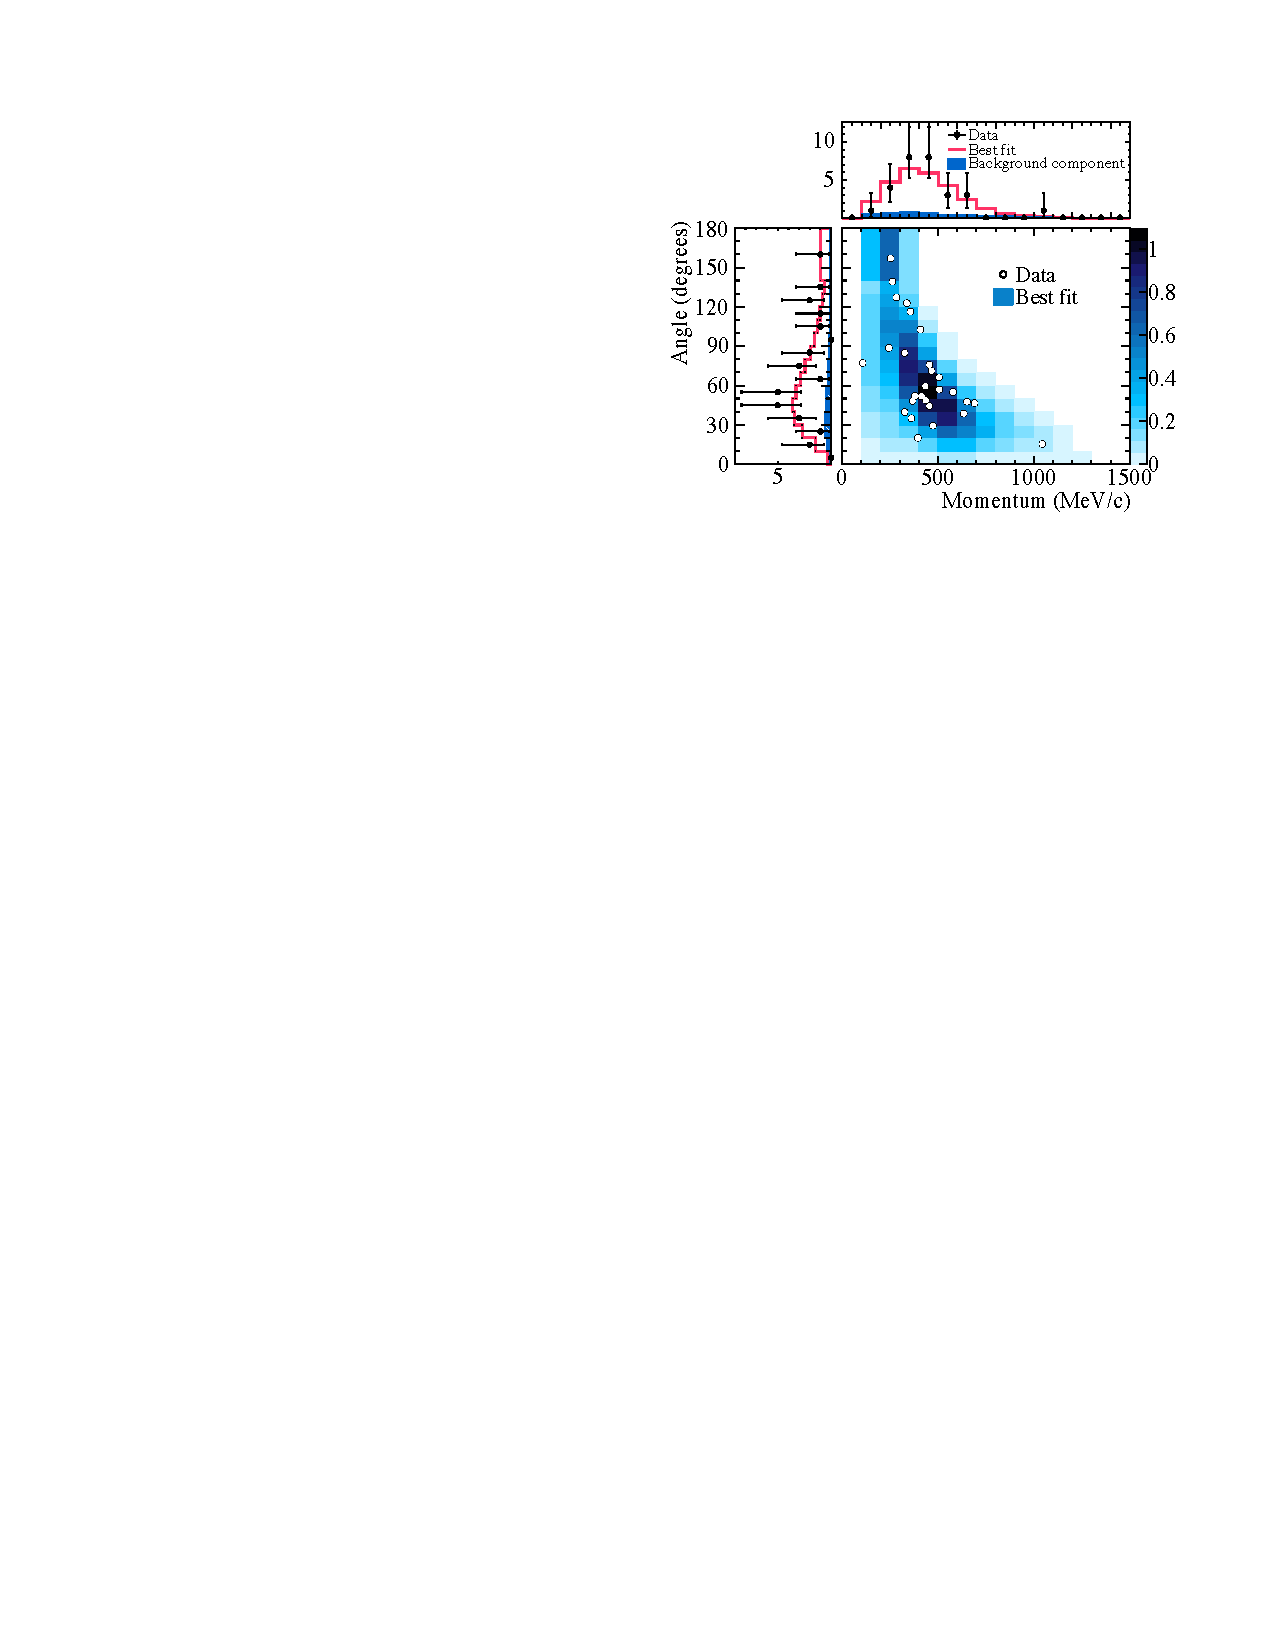
\includegraphics[width=14cm]{figures/nueapp_ptheta.pdf}
\caption{\label{fig:t2kapp} \ptheta distribution for the \nue candidates events. Courtesy of the T2K collaboration.}
\end{center}
\end{figure}



%%%%


In the coming years, before new projects, that will be described in~\ref{sec:future}, will come online, the quest for the missing parameters in the PMNS scheme (\dcp, mass ordering, \thatm octant) will be led by the two long-baseline accelerator experiments that are currently taking data, namely T2K and NOVA.

T2K has recently published its first analysis of neutrino oscillations obtained combining data taken with neutrinos and antineutrinos beam with approximately the same amount of POT\cite{t2k2016}. With this data set 32 e-like candidates are observed at SK in neutrino mode and 4 in antineutrino mode. The expected number of events depends on the value of \dcp and of the mass ordering as shown in Table~\ref{tab:evtnue}, varying between 19.6 and 28.7 (17.1 and 25.4) for normal (inverted) ordering in neutrino mode and between 6.0 and 7.7 (6.5 and 7.4) in antineutrino mode. The value $\dcp=-\pi/2$ maximize the \nue appearance probability and minimize the \nueb appearance probability while the opposite happens for $\dcp=\pi/2$. 

\begin{table}[htbp]
    \centering
    \caption{Number of $\nu_e$ and $\overline{\nu}_e$ events expected for various values of $\delta_{CP}$ and both mass orderings 
    compared to the observed numbers.}
    \label{tab:evtnue}
    \begin{tabular}{|c|c|c|c|c|c|}
        \hline
        Normal & $\delta_{CP}= -\pi/2$ & $\delta_{CP}= 0 $ & $\delta_{CP}= \pi/2$ &  $\delta_{CP}= \pi$  & Observed\\
        \hline 
        $\nu_e$ &   28.7 & 24.2& 19.6& 24.1& 32 \\
        $\overline{\nu}_e$ &  6.0 &6.9& 7.7 &6.8 &4 \\     
        \hline
        \hline
        Inverted & $\delta_{CP}= -\pi/2$ & $\delta_{CP}= 0 $ & $\delta_{CP}= \pi/2$ &  $\delta_{CP}= \pi$  & Observed\\
        \hline 
        $\nu_e$ 			& 25.4 	& 21.3	& 17.1	& 21.3	& 32 \\
        $\overline{\nu}_e$ 	& 6.5 	& 7.4		& 8.4		& 7.4		&4 \\    
\hline
    \end{tabular}
\end{table}


Since T2K observes a mild excess of \nue candidates with respect to the most favourable value and a deficit of \nueb candidates, a value of \dcp close to $-\pi/2$ and the normal ordering is preferred by these data even without the inclusion of the reactor constraint for the measurement of \thint. This is shown in Fig.~\ref{fig:t2kjoint}. For the first time, long-baseline experiments have sensitivity to \dcp without considering independent informations from reactors and a good agreement between the value of \thint measured by the reactors and the one measured by T2K is observed. 

\begin{figure} [htbp!]
\begin{center}
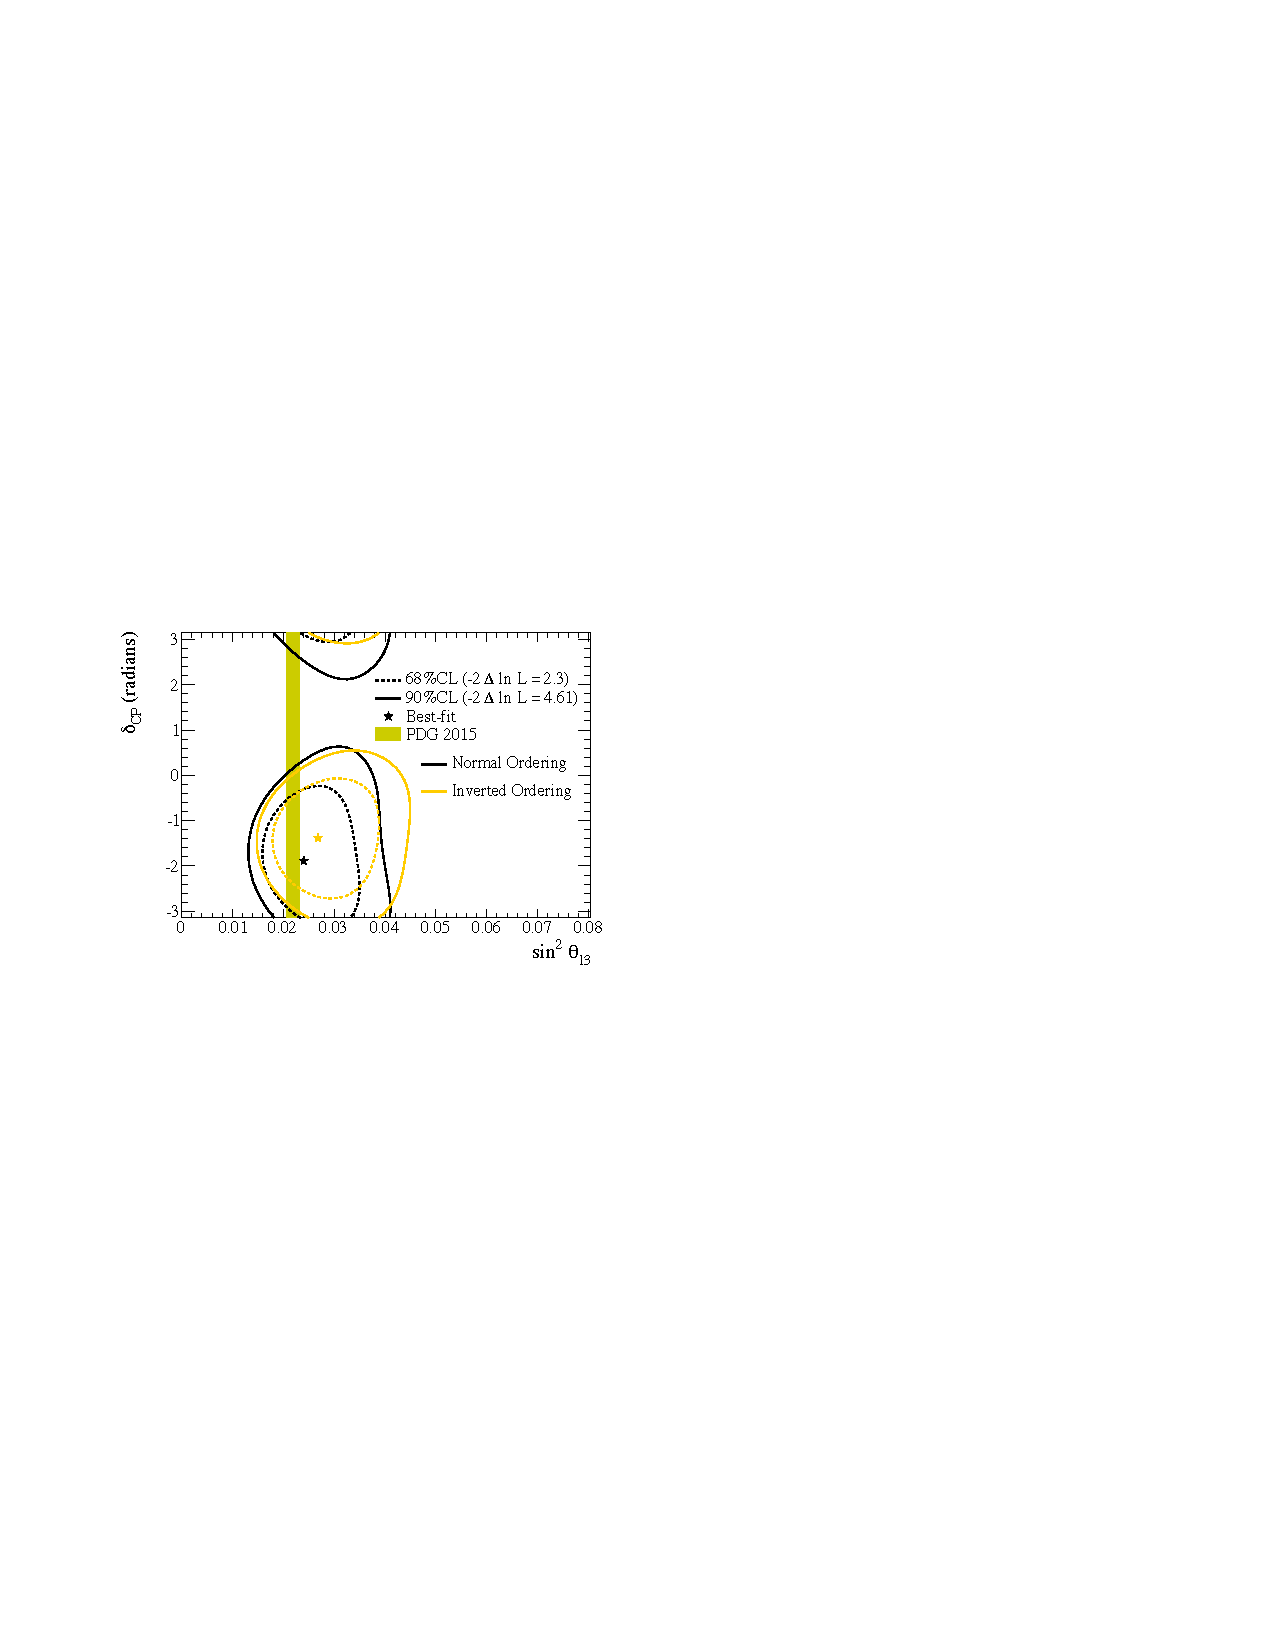
\includegraphics[width=10cm]{figures/t2k_joint_th13dcp.pdf}
\caption{\label{fig:t2kjoint} 68\% and 90\%  constant $-2\Delta ln L$ in the \dcp - \sto plane are shown by the dashed
(continuous) lines, computed independently for the normal
(black) and inverted (yellow) mass ordering. The best-fit point
is shown by a star for each mass ordering hypothesis. The
68\% confidence region from reactor experiments on \sto is
shown by the yellow vertical band. Courtesy of the T2K collaboration.}
\end{center}
\end{figure}


When the average value of \thint as measured by the reactor experiments is used additional informations on the value of \dcp can be obtained. The T2K collaboration has obtained confidence intervals for \dcp using the Feldman-Cousins method (see Fig.~\ref{fig:t2kdcp}) and values conserving CP (\dcp=0 or $\pi$) are excluded at 90\% C.L.

\begin{figure} [h!]
\begin{center}
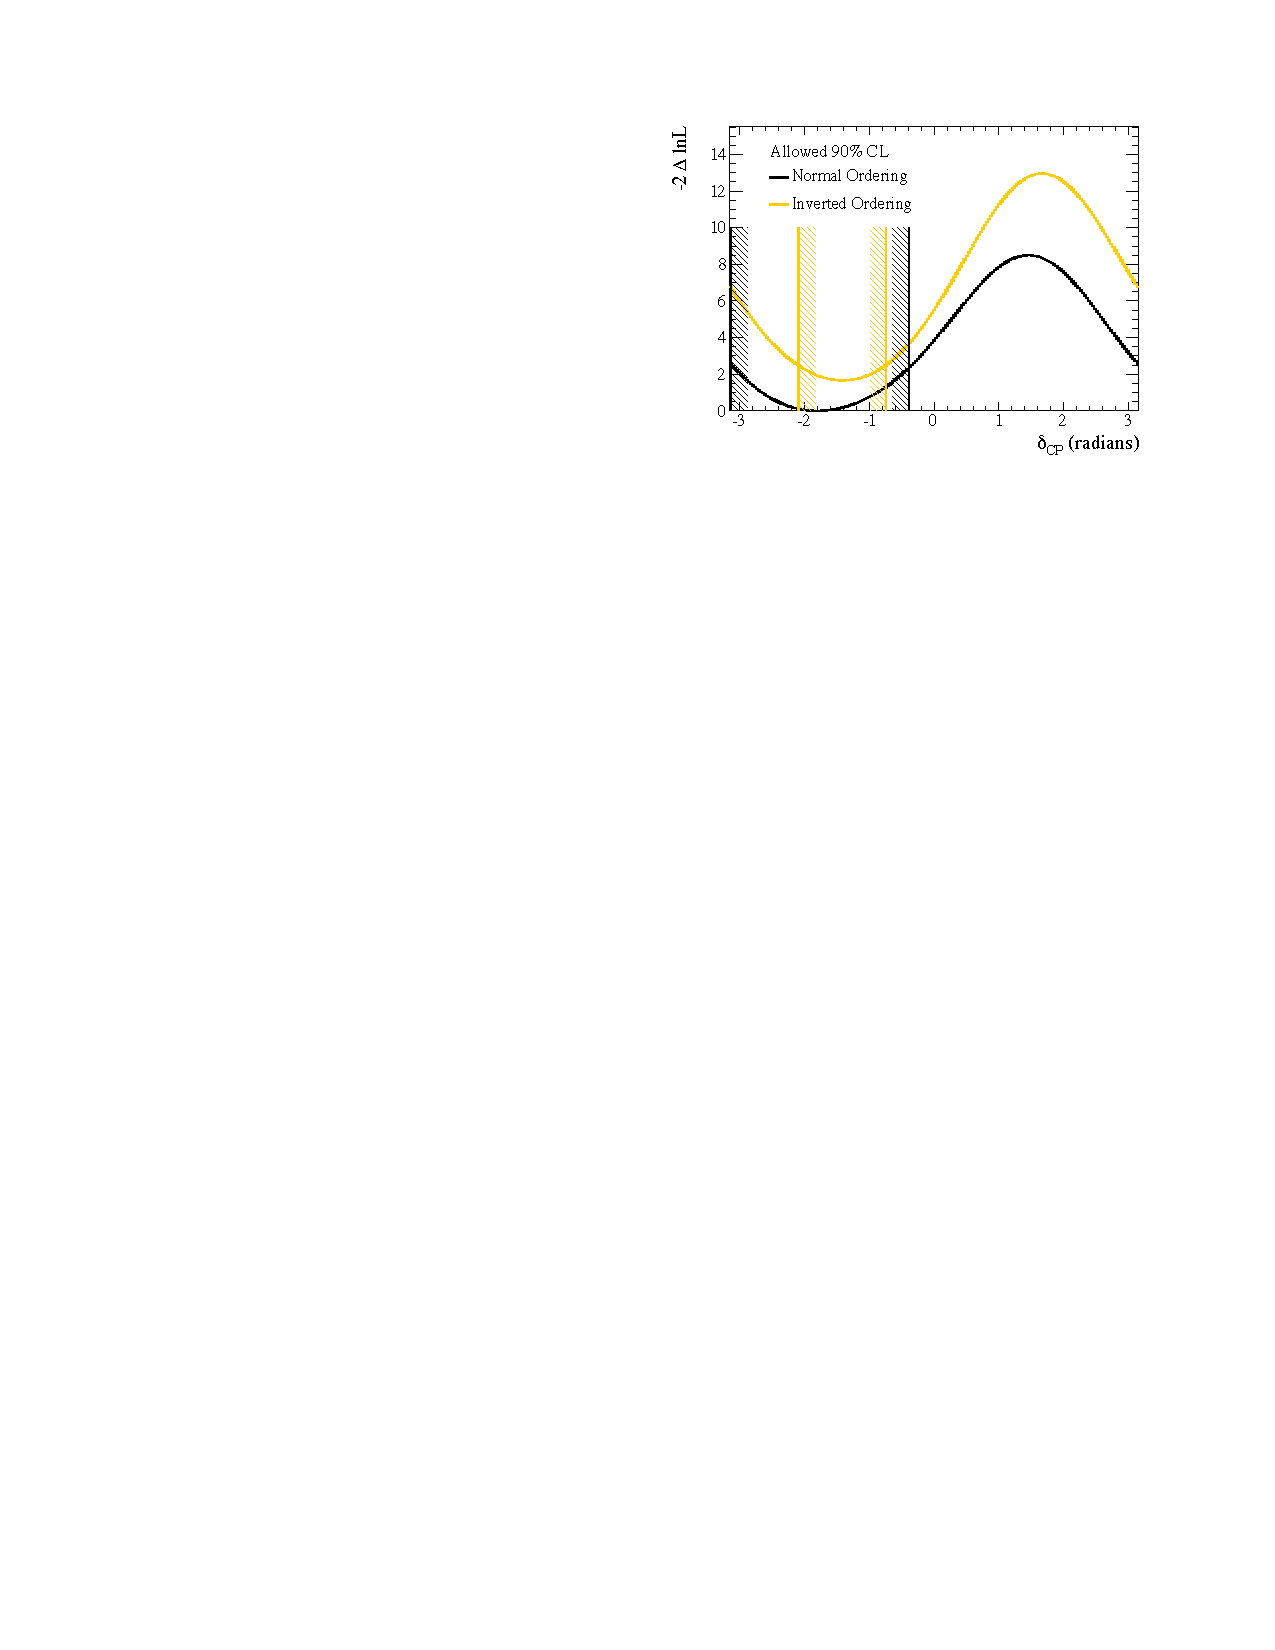
\includegraphics[width=10cm]{figures/t2k_dcp_1D.pdf}
\caption{\label{fig:t2kdcp}$-2\Delta ln L$  as a function o \dcp for the normal (black)
and inverted (yellow) mass ordering. The vertical lines show the
corresponding allowed 90\% confidence intervals, calculated
using the Feldman-Cousins method and \sto is marginalised
using the reactor measurement as prior probability. Courtesy of the T2K collaboration.}
\end{center}
\end{figure}

 
\nova has also released new results for the \nue appearance (they did not collected data with antineutrino yet). They observed 33 \nue candidates events at the far detector with $8.2\pm0.8$ background events expected. The prediction for the signal events vary from 28.2 (Normal Ordering, $\dcp=-\pi/2$) to 11.2 (Inverted Ordering, $\dcp=\pi/2$). A joint analysis of appearance and disappearance channels has not been released by \nova yet but using the constraints from their own disappearance sample the results in the \stt-\dcp plane is shown in Fig.~\ref{fig:novadcp}. The data have a mild preference for normal ordering, non-maximal values of \stt. \nova foresee to start taking data in antineutrino mode in 2017 and those data will help in solving the degeneracies shown in Fig.~\ref{fig:novadcp}. 

\begin{figure} [htbp!]
\begin{center}
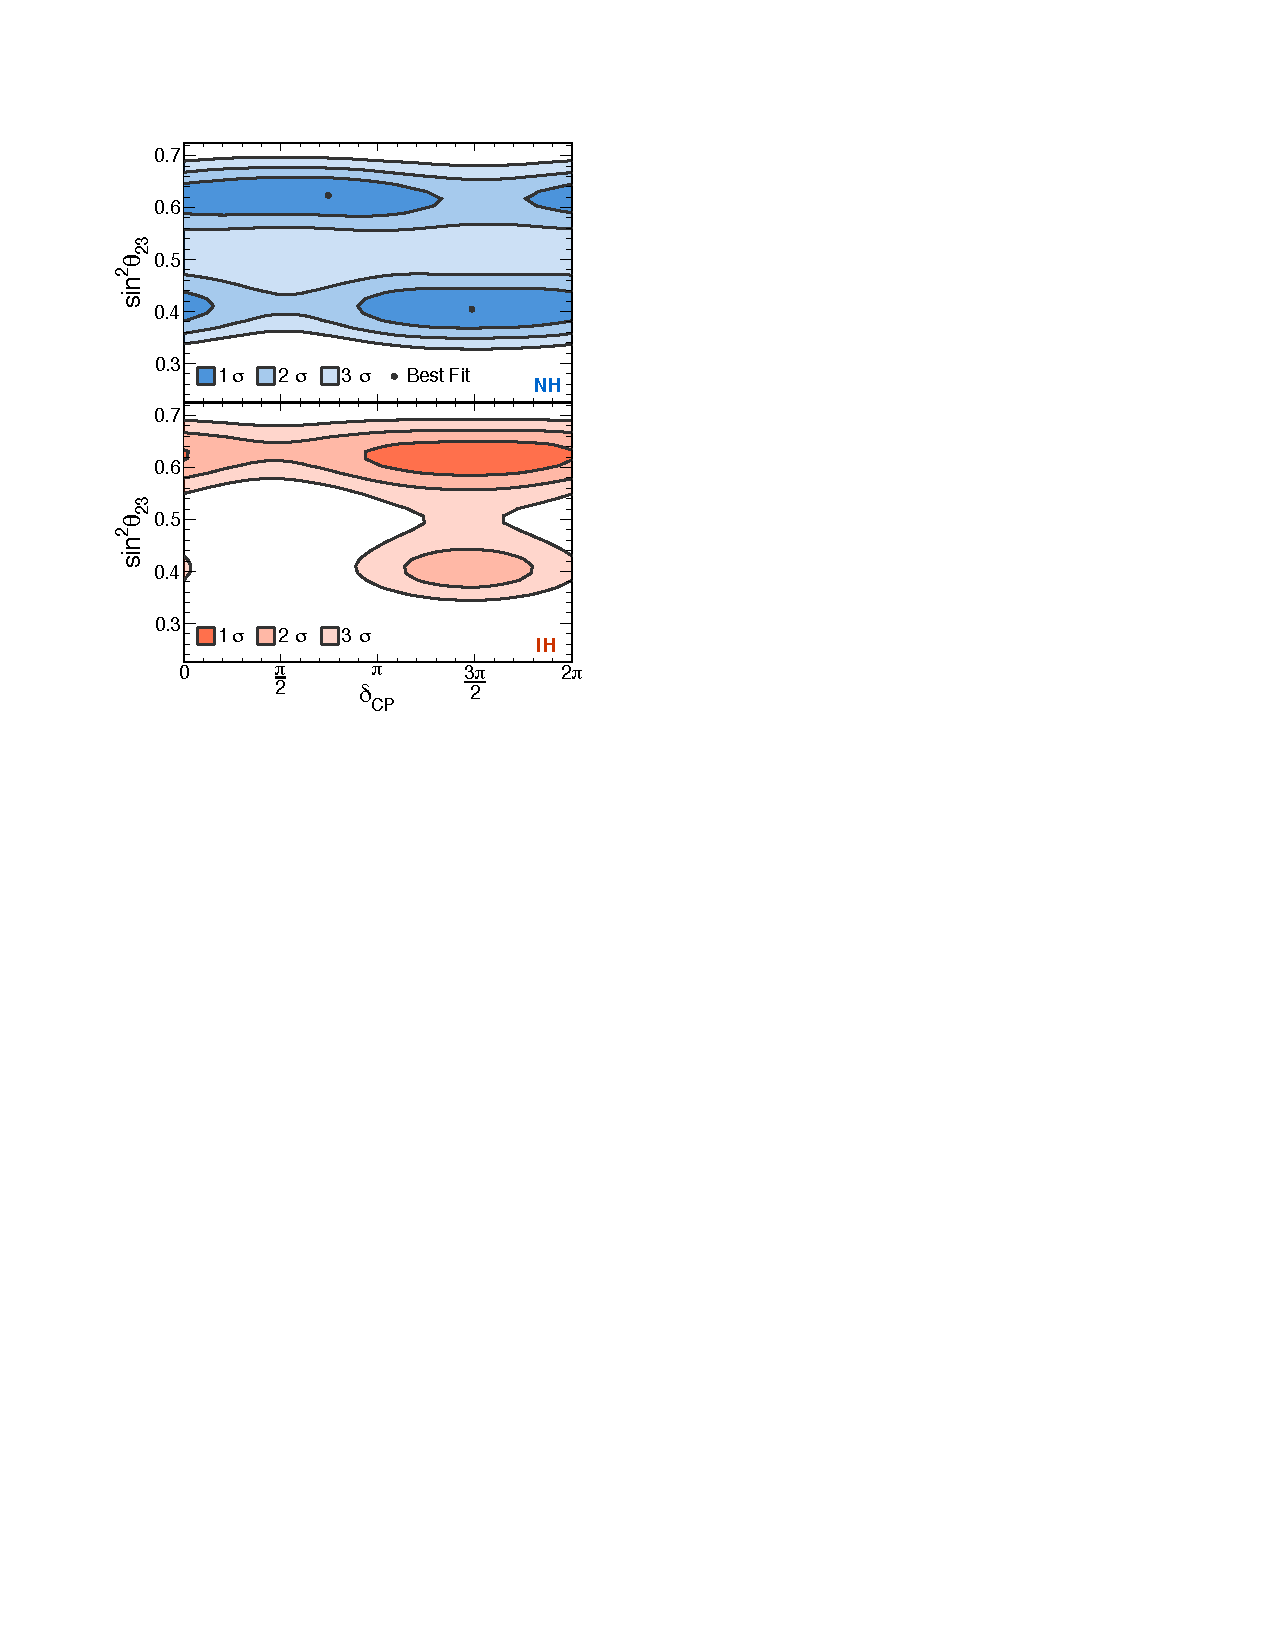
\includegraphics[width=10cm]{figures/nova_nueappearance.pdf}
\caption{\label{fig:novadcp}  Regions of \dcp versus \stt consistent with the observed spectrum of \nue and \num candidates in \nova. The top panel corresponds to normal mass ordering and the bottom panel to inverted hierarchy~\cite{Adamson:2017gxd}.}
\end{center}
\end{figure}



%\subsection{ Search for \dcp and 3-nu effects in atmospheric neutrinos (SK)}
%SK effect in atm due to delta
%(look for a reference)